

\begin{figure*}[!t]
\centering
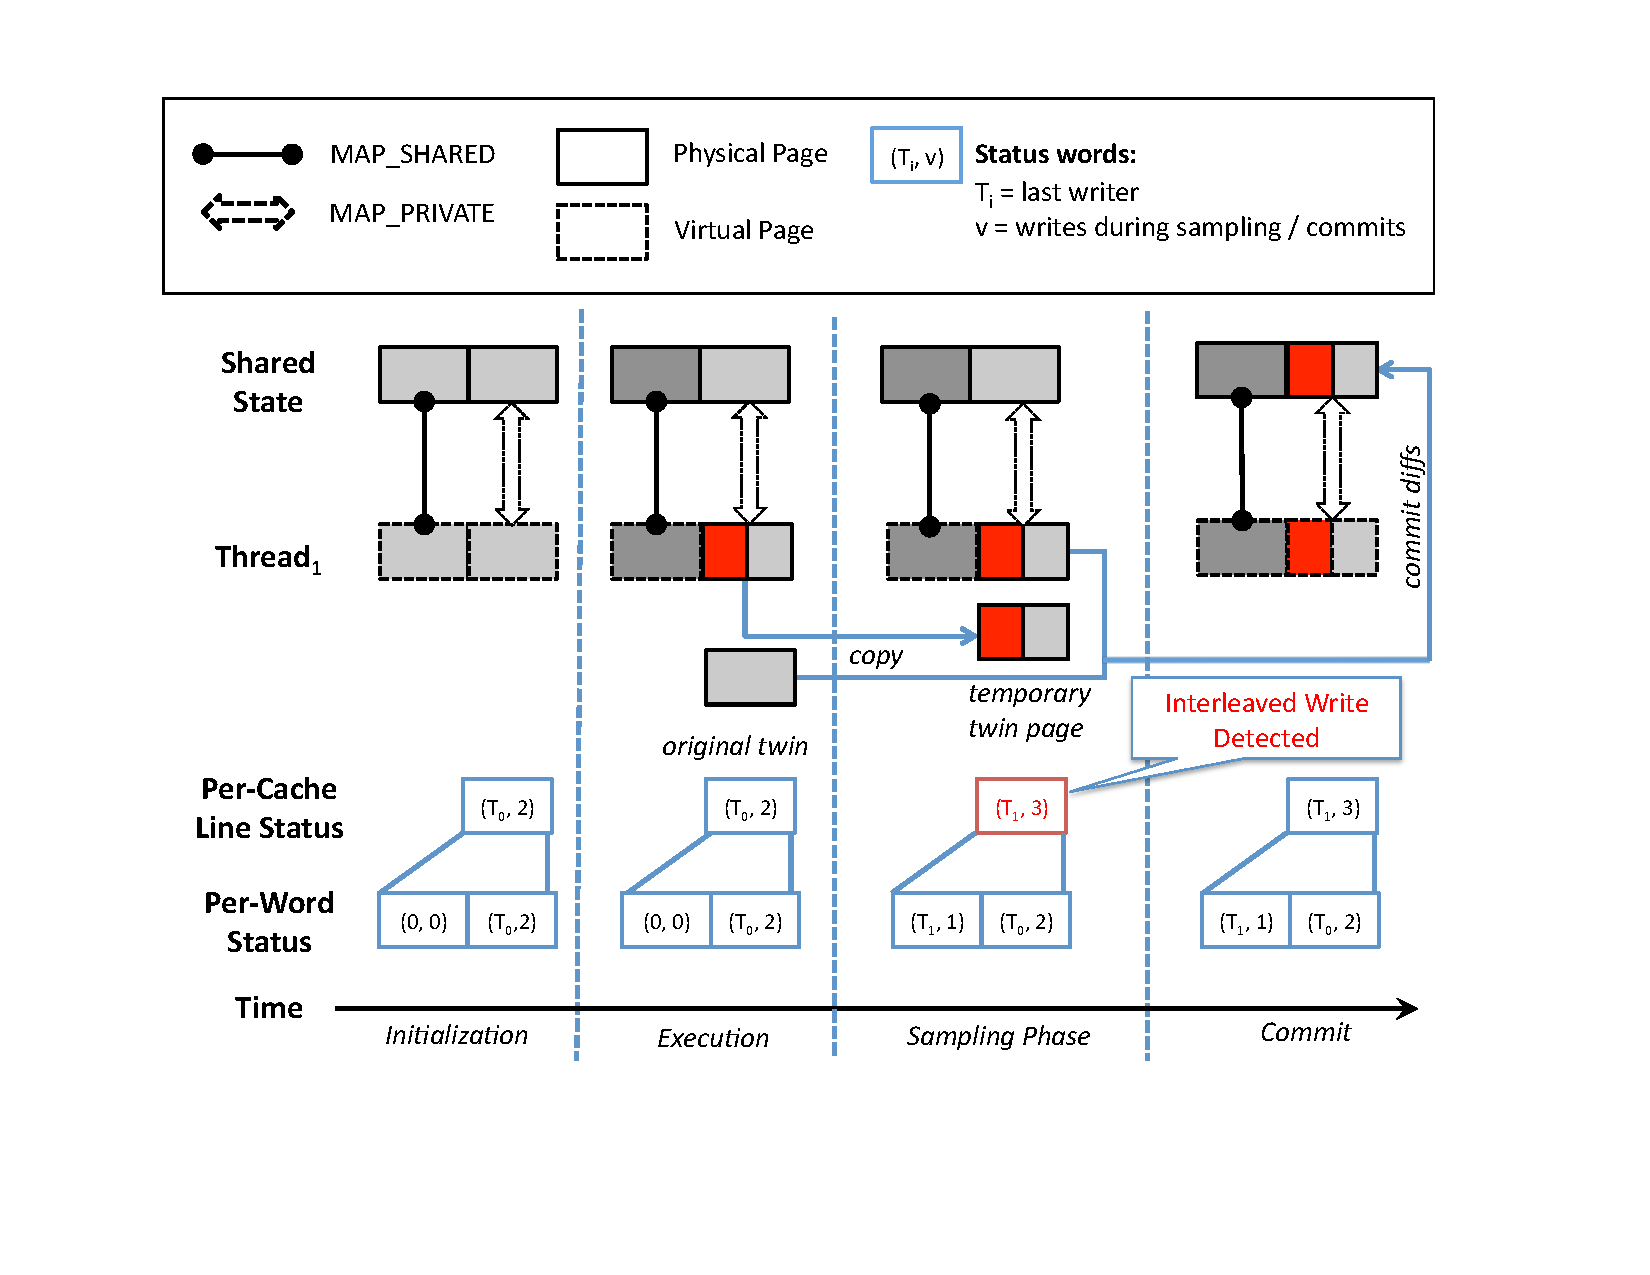
\includegraphics[width=6in]{figure/sheriffdetective}
\caption{
Overview of \sheriffdetect{}'s operation.
\sheriffdetect{} extends \sheriff{} with page ownership tracking, sampling,
and  \emph{per-cache line and per-word status} arrays
that track frequent false sharing
within cache lines. For clarity of exposition, the diagram depicts just one cache line per page and two words per cache line.
\label{fig:detectiveoverview}}
\end{figure*}

\label{sec:falseshare}

We use the \sheriff{} framework to build two
tools that address false sharing. This section
describes the first of these, \sheriffdetect{}, which detects false sharing.

\sheriffdetect{} detects both types of false sharing described in
the literature. The first is the sharing of structurally-unrelated
objects that happen to be located on the same cache line (i.e.,
different variables). The second is when multiple processors access
different fields of the same object, which Hyde and Fleisch describe
as ``pseudo sharing''~\cite{falseshare:Analysis}.

\sheriffdetect{} is designed to report only those instances of false sharing with
the potential to seriously degrade performance. False sharing
only causes a significant performance degradation when multiple threads
concurrently and repeatedly update falsely-shared data, leading to
large numbers of invalidation misses.

\subsection{Page Ownership Tracking}
\label{falseshare:basic mechanism}

One approach to implementing \sheriffdetect{} would be to use \sheriff{} and direct it to 
protect all pages and map them private.
The only change needed to detect false sharing would be an added check of twins
and diffs against committed pages. Any cache line whose contents
differ from the twin indicates it was changed by another thread. False sharing
has occurred whenever a diff (a
local update) lies on the same cache line as a local update.

However, this na\"{\i}ve approach would be quite costly. Since all local
modifications of different threads must be committed to the shared
space at every synchronization point to ensure correct
execution (see Section~\ref{simulation:syn}), this approach would
introduce substantial and unnecessary overhead for applications with a
large number of unshared pages.

To reduce this overhead, \sheriffdetect{} leverages a simple insight:
if two threads can falsely share a cache line, then
they must simultaneously access the page containing that
cache line.

Guided by this insight, \sheriffdetect{} relies on page protection to
gather information about whether pages are shared or not.
Instead of placing everything in the private address space,
\sheriffdetect{} utilizes its knowledge about page sharing patterns and
only maps those shared pages private.

\sheriffdetect{} initially read-protects all memory pages
and tracks the number of threads that attempt to write a page concurrently.
Any attempt to write to a
page will trigger a page fault.
\sheriffdetect{} then
increments the access counter for this page before unprotecting the page.
Once the access counter for a given page reaches two,
the page is considered to be shared,
and the page is mapped privately to each process to allow \sheriffdetect{} to locate possible false sharing.

% The protection can be done both in the periodic timer handler and at the end of one transaction.

\subsection{Discovering Local Modifications}
\label{falseshare:memorywrites}

When \sheriffdetect{} concludes each transaction, it compares each dirty page
with its twin a word at a time to find any modifications. \sheriffdetect{} thus
identifies all writes made by the current thread. 
Whenever local modifications are found, either in the sampling period or
at the end of a transaction (outside a critical section), \sheriffdetect{}
sets the virtual status words that indicate local modifications by the
current thread.

\subsection{Identifying Problematic False Sharing}
\label{detection:sampling}

\sheriffdetect{} uses sampling to measure the performance impact of
false sharing, which it uses to rank its reports.  \sheriffdetect{}
currently uses a sampling interval of 10 milliseconds, which we
empirically observe balances accuracy and performance overhead.

\sheriffdetect{} tracks the frequency of updates made to cache lines
by associating a temporary twin page with each private, modified page
(see Figure~{\ref{fig:detectiveoverview}}). These temporary twins are
created only during sampling, and are updated to reflect the current
working version at every sampling interval.

\label{detection:invalidation}

Only repeatedly interleaved writes (that is, by different threads) can
degrade performance by repeatedly forcing cache line
invalidations.  \sheriffdetect{} monitors interleaved writes across
different threads in order to capture this effect.

\sheriffdetect{} associates a \emph{per-cache line status} with
each cache line in every tracked page
(Figure~\ref{fig:overview}). This status contains two fields. The
first points to the last thread to write to this cache line, and the
second records the number of interleaved updates to the cache line.
Every time a different thread writes to a cache line, \sheriffdetect{}
updates the associated status word with both the thread id and the
version number. To reduce overhead, \sheriffdetect{} splits the
status into two different arrays to allow the use of atomic operations
instead of locks.

In addition, during sampling and at commit time, \sheriffdetect{}
updates \emph{per-word status} values for every modified word. This
information is later used to report the approximate frequency of
updates at the individual word granularity. Programmers can then use
this information to decide where to place padding. For example, if two
struct fields are falsely shared, padding should be placed
between the fields that are most frequently updated.

\sheriffdetect{} imposes relatively low memory overhead by maintaining
status values only for pages that are shared by multiple threads. To
further save space, \sheriffdetect{} stores each status in a single
32-bit word. The upper 16 bits stores the thread id, and the lower 16
bits stores the version number. When a word is detected to have been
modified by more than two threads, \sheriffdetect{} sets the thread id
field to \texttt{0xFFFF}, indicating that it is shared.

%  The \texttt{CacheInvalidation}
%array capture those interleaving cache invalidation for all
%cache lines in protected memory.  Every cache line has a corresponding
%counter to indicate the interleaving of cache invalidation for this
%cache line.  LastThreadModifyCache array is used to record last thread
%id to write on its cache line.


\subsection{Reporting}

\label{detection:object}

At this point, \sheriffdetect{} has detected individual cache lines that
are responsible for a large number of invalidations, and thus potential
sources of slowdowns. The next step is to identify the culprit objects.

\sheriffdetect{} aims to provide as much
context as possible about false sharing in order to reduce programmer
effort, identifying global variables by name, heap objects by
allocation context, and where possible, the fields modified by
different threads.
\sheriffdetect{} also provides an option to print out detailed information for every word in a
given cache line, including the number of updates and the accessor threads.

\sheriffdetect{} identifies globals directly by using debug
information that associates the address with the name of the
global. For heap objects, \sheriffdetect{} instruments memory
allocation to attach the call site to the header of each heap
object. This calling context indicates the sequence of function calls
that led to the actual allocation request, and is useful to help the
programmer identify and correct false sharing, as the case
study in Section~\ref{evaluation:comparison} demonstrates. Any heap
object responsible for a large number of invalidations is not
deallocated so that it can be reported at the end of program
execution.

\subsection{Avoiding False Positives}
\label{detection:avoidfalsepositive}

\sheriffdetect{} instruments memory allocation operations to
clean up cache invalidation counts whenever an object is
de-allocated. This approach avoids the false positives caused by
incorrectly aggregating counts when one address is re-used for other
objects.

\subsection{Reporting Falsely Shared Objects}

Once execution is complete, \sheriffdetect{} generates a ranked list of
falsely shared objects.  \sheriffdetect{} scans the cache invalidation
array for cache lines with a number of invalidations above a fixed
threshold (currently 100).  The corresponding invalidation times and
offset of this cache line are added to a global linked list sorted by
invalidation times.

After scanning the cache invalidation array, \sheriffdetect{} obtains object
information for all cache lines in the linked list, and reports
the allocation site and offsets of all falsely-shared allocated objects.

\subsection{Optimizations}

\sheriffdetect{} employs several optimizations that further reduce its overhead.

\paragraph{Reducing timer overhead.} 
As explained in Section~\ref{detection:sampling},
\sheriffdetect{} uses sampling to track 
interleaved writes by triggering a timer signal via \texttt{ualarm}. To reduce the
impact of timer interrupts, \sheriffdetect{} activates sampling
only when the average transaction time is larger than a threshold time
(currently 10 milliseconds). \sheriffdetect{} uses an exponential moving
average to track average transaction times ($\alpha = 0.9$). This
optimization does not significantly reduce 
the possibility of finding false sharing since
\sheriffdetect{}'s goal
 is to find an object with a large amount of interleaved
writes from different threads.

\paragraph{Sampling to find shared pages.} \sheriffdetect{} relies on
page protection to determine whether pages are shared or not. When one
application has a large number of transactions or page touches, the
protection overhead to gather this sharing information can dominate running
time.

\sheriffdetect{} reduces overhead by using sampling to detect shared
pages. If objects on a page are frequently falsely shared, the page
itself must also be frequently shared, so even relatively infrequent
sampling will eventually detect this sharing.  \sheriffdetect{}
currently samples the first 50 out of every 1,000 periods (one period
equals one transaction or one sampling interval). At the beginning of
each sampled period, all memory pages are made read-only so that any
writes to each page will be detected.  Once a page is found to be
shared, \sheriffdetect{} will track any false sharing inside it.
\sheriffdetect{} only updates the shared status of pages during
sampled periods and at commit points. During unsampled periods, pages
whose sharing status is unknown impose no protection overhead.

\subsection{Discussion}

Unlike previous tools, \sheriffdetect{} has no false positives, differentiates true sharing from
false sharing, and avoid false positives caused by the reuse of heap objects.
\sheriffdetect{} can under-report false sharing instances in the following situations:

\paragraph{Single writer.}
False sharing usually involves updates from multiple threads, but it
can also arise when there is exactly one thread writing to part of a
cache line while other threads read from it. Because its detection
algorithm depends on multiple, differing updates, \sheriffdetect{} cannot
detect this kind of false sharing.

\paragraph{Heap-induced false sharing.}  \sheriff{} replaces the standard
memory allocator with one that behaves like Hoard and thus reduces the
risk of heap-induced false sharing. \sheriffdetect{} therefore does
not detect false sharing caused by the standard memory allocator.
Since it is straightforward to deploy Hoard or a similar allocator
to avoid heap-induced false sharing, this limitation is not a problem
in practice.

%Besides, using some Hoard-like memory allocator can be very helpful to improve the performance of multi-threaded programs
%and that should be the standard for memory allocator for multi-threaded programs.

\paragraph{Misses due to sampling.}  Since it uses sampling to
  capture continuous writes from different threads, \sheriffdetect{} can
  miss writes that occur in the middle of sampling intervals. We
  hypothesize that false sharing instances that affect performance are
  unlikely to perform frequent writes exclusively during that time, and so
  are unlikely to be missed.
